\chapter{Marco Teoríco}

En este capítulo veremos los principales conocimientos que son necesario para el entendimiento del presente seminario.
\section{Conceptos previos}
\subsection{CPU}(Central Processing Unit) es el hardware encargado del procesamiento de tareas mediante las operaciones básicas aritméticas, logicas y de entrada y salida del sistema. Los ordenadores actuales cuenta con más de una lo cual les permite usar multiprocesamiento. Los nucleos de la cpu estan hechos para el procesamiento de las tareas de manera secuencial.
Una CPU tiene 2 componentes principales:
+ **ALU (Unidad Aritmetica Logica):** se encarga de realizar las operaciones aritméticas y lógicas.
+ **CU  (Unidad de Control       ):** extrae información de la memoria la decodifica y ejecuta llamando a ALU las veces que sea necesario.

\subsection{GPU}
Las GPU(Graphics Processing Unit)
A diferencia de las CPU los GPU's estan compuestos de miles de nucleos que fueron diseñados para resolver tareas en paralelo.

\subsection{GPGPU} 
GPGPU(General Purpose Graphics Processing Unit) consiste en realizacción de los calculos que comumente serian realizados por el CPU utilizando GPU. Este método permite aprovechar los beneficios de potencia en procesamiento paralelos de las GPU's.
\begin{figure}[H]
	\centering
	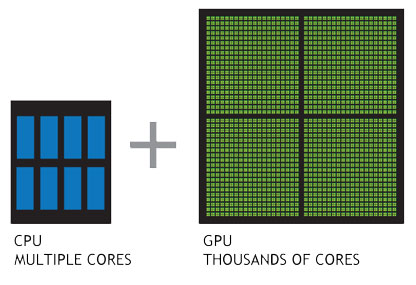
\includegraphics[width=0.9\textwidth]{Figures/cpu-and-gpu.jpg}
	\caption{Esquema GPGPU}
	\label{MVC}
\end{figure}



\section{Metodología}
ASDFASDFASDFA

\subsection{SCRUM}

ASDFASDFASDFA


\subsubsection*{Características}

\begin{figure}[H]
\centering
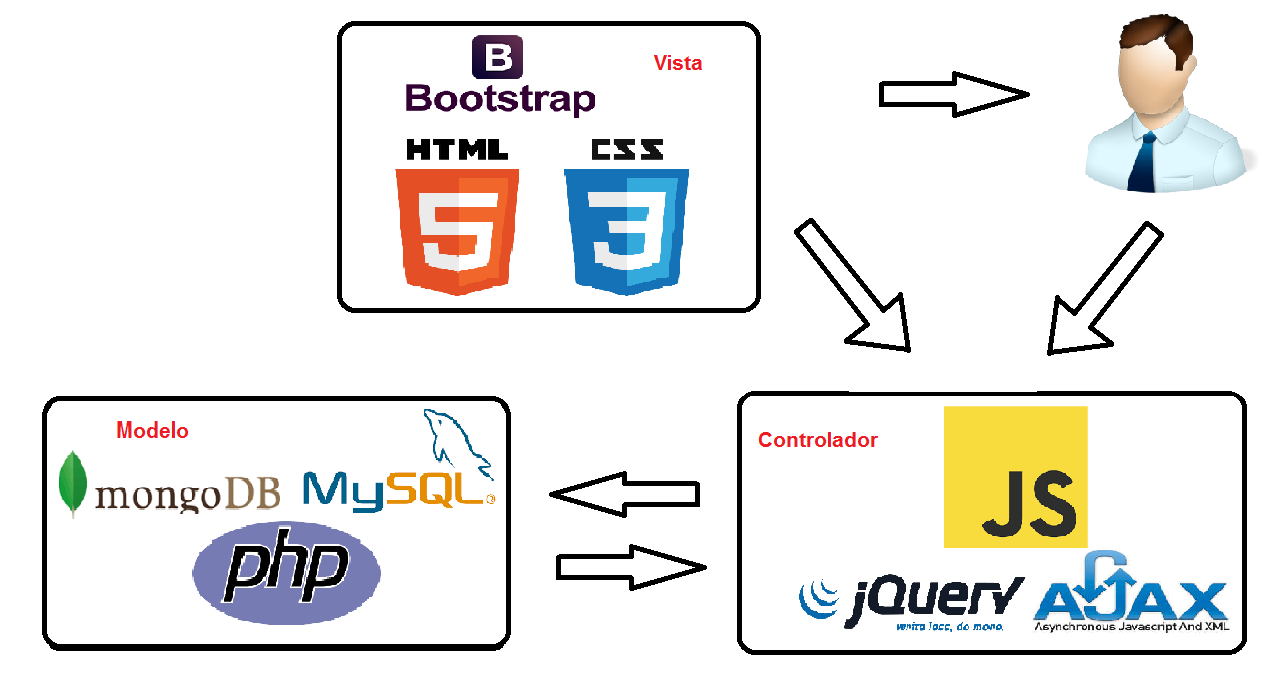
\includegraphics[width=0.9\textwidth]{Figures/mvc.png}
\caption{Modelo-Vista-Conrolador}
\label{MVC}
\end{figure}


\afterpage{\blankpage}